\chapter{parxpaMcada atuyxnanxta maTaTxda vijAcnxni AyaRBaTa}%%%2

\begin{wrapfigure}{r}{0.4\textwidth}
  \centering\includegraphics[scale=0.8]{src/figures/aryabhata.eps}
  
  {\bf AyaRBaTa}
    \end{wrapfigure}


%\begin{figure}[H]
%\centering\includegraphics[scale=0.8]{src/figures/aryabhata.eps}
%\end{figure}
halavAru hosa parxyoVgagaLanunx, halavu mUla aBipArxyagaLanunx parxpaMcakekx modala sala koTaTx BAratiVya budidhxvaMta sherxVSaThxru, kirx.sha.~{\rm 400} riMda {\rm 1200}ra varegina sumAru {\rm 800} vaSaRgaLa avadhiyalilxdadx meVdhAvigaLu.

kirx.sha.~{\rm 5}neya shatamAnadiMda kirx.sha. {\rm 7}neya shatamAnadavaregina kAlavanunx BAratiVya\break KagoVLa matutx gaNita shAsatxrXgaLa savxNaRyuga eMdu kelavaru aBipArxyapaDutAtxre.

kirx.sha.~{\rm 5}neya shatamAnadalilxdadx kusumApurada AyaRBaTa, {\rm 6}neya shatamAnada\break varAhamihira matutx {\rm 7}neya shatamAnada barxhamxgupatx matutx modalaneya BAsakxra ivaralilx muKayxru.

gaNita matutx KagoVLavijAcnxnagaLige oMdu vayxvasithxta hAgU veYjAcnxnikamAgaR\-vanunx toVrisikoTaTx kiVtiR hAgU gaNita matutx KagoVLajacnxra aneVka AviSAkxragaLige modaliga eMba kiVtiRyU AyaRBaTarige salulxtatxde.

parxpaMcada sherxVSaThxmaTaTxda vijAcnxnigaLa peYki kirx.sha. {\rm 499}ralilx `AyaRBaTiVyaM' bareda BAratiVya gaNitajacnx hAgU KagoVLatajacnx AyaRBaTarU obabxru.

AyaRBaTiVyaMdalilx Eka ({\rm 1}), dasha ({\rm 10}), shata ({\rm 100}), sahasarx ({\rm 1000}), Ayuta ({\rm 10,000}), niyuta ({\rm 1,00,000}), parxyuta ({\rm 10,00,000}), koVTi ({\rm 1,00,00,000}), nayxbuRda athavA nUru koVTi - iMtha dashamAna padadhxti tiLisuva {\rm 18} sAthxnagaLu gurutisalapxTiTxve.


AyaRBaTaru gaNita, kAlakirxyA, goVlamf eMba mUru BAgagaLanunx tananx garxMtha `AyaRBaTiVyaM'nalilx parxsAtxpisidAdxre.

AyaRBaTaru viSayagaLanunx nAlukx pAdagaLAgi viBAgisidAdxre.
\begin{itemize}
\item[{\rm 1)}] {\bf giVtikApAda:} idaralilx {\rm 13} sholxVkagaLive. idaralilx KagoVLavijAcnxnakekx saMbaMdhisida kelavu muKayxvAda bele matutx lekAkxcAragaLanunx sUtarxda rUpadalilx koDalAgide.

\item[{\rm 2}] {\bf gaNitapAda:} idaralilx {\rm 33} sholxVkagaLive. idaralilx vagaRmUla, GanamUla tirxBujada keVtarxPala (sale), vaqtatxda sale, sherxVDhiVgaNita, vagaRsamiVkaraNa, kuTaTxka matutx vagaR, anidiRSaTx samiVkaraNagaLu, shaMkuvina neraLugaLa lekakxgaLu, terxYrAshi muMtAda viSayagaLa bagegx vivaraNeyide. 
  
\item[{\rm 3}] {\bf kirxyApAda:} idaralilx {\rm 25} kArikegaLive. idaralilx kAlada viBAgagaLu sUyaR, caMdarx matutx itara garxhagaLa sAthxnagaLa niSakxsheR, vividha mAsa saMvatasxragaLu muMtAda viSayagaLive.
 
\item[{\rm 4}] {\bf goVlAdhAyxya:} idaralilx $50$ kArikegaLive. idaralilx BUmi guMDAgiru\-vudu. adu parxtidina tananx akaSxda meVle tirugutitxruvudariMda sUyoVR\-daya, sUyARsatxgaLu uMTAgutitxruvudu. BUmi matutx itara garxhagaLu savxyaM parxkAsha vasutxgaLalalx, BUmi pashicxmadiMda pUvaRda kaDege tirugutitxde - I parxsAtxpagaLelalx ive.
  \end{itemize}

%\eject

\noindent
{\bf KagoVLavijAcnxnakekx AyaRBaTara mahatatxvXda koDugegaLeMdare:}

\begin{itemize}
\item[{\rm 1)}] BUmiya AkAra matutx calane
  
\item[{\rm 2)}] sUyoVRdaya matutx sUyARsatx beVre beVre jAgagaLalilx beVre beVre kAlakekx uMTAgutatxve.
  
\item[{\rm 3)}] BUmiya utatxra dhurxva matutx dakiSxNa dhurxvaparxdeVshagaLalilx Aru tiMgaLu hagalu matutx Aru tiMgaLu iruLu irutatxve.

\item[{\rm 4)}] mahAyugaveMba oMdu diVGaRkAlavadhiyalilx oMdoMdu AkAshakAya eSeTxSuTx pariBarxmaNegaLanunx pUtiRyAgi mugisutatxde eMba saMKeyxgaLanunx koTiTxdAdxre. mahAyugada badalu kalapx eMba shabadx parigaNisi A avadhiyalilx garxhagaLa pariBarxmaNa saMKeyxgaLanUnx niVDidAdxre. 

\item[{\rm 5)}] saMparxdAyadiMda baMdidadx yuga sidAdhxMtavanunx biTuTx sulaBavAda matutx garxha gaNitada lekAkxcAragaLige anukUlavAguva hosa riVtiya yugaviBajaneyanunx yoVcisidAdxre. 

\item[{\rm 6)}] eraDu garxhagaLu edurubadurAgi calisutitxdadxre A eraDara aMtaravanunx avugaLa veVgagaLa motatxdiMda BAgisi, oMdeV dikikxnalilx calisutitxdadxre avugaLa aMtaravanunx veVgagaLa vayxtAyxsadiMda BAgisidare Aga baruva BAgalabadhxvu A eraDu garxhagaLu saMdhisuva athavA saMdhisada a naMtarada kAlAvadhiyanunx koDutatxde.
\begin{figure}[H]
\centering
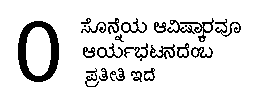
\includegraphics[scale=0.8]{src/figures/fig17.eps}
\end{figure}
   
  
\item[{\rm 7)}] oMdu mahAyugada kAlAvadhiyalilx, BUmiyiMda viVkiSxsidAga sUyaR, caMdarx, garxhagaLu eSeTxSuTx pariBarxmaNegaLanunx pUreYsutatxve eMbudanunx koTiTxdAdxre. 

%\eject

\item[{\rm 8)}] caMdarxgarxhaNa matutx sUyaRgarxhaNagaLu saMBavisalu veYjAcnxnika kAraNa\-gaLanunx suPxTavAgiyU, saMkeSxVpavAgiyU tiLisidAdxre. 
  
\item[{\rm 9)}] sUyaR caMdArxdigaLa suPxTasAthxnagaLanunx viVkaSxNeyiMda tALe noVDalu saMkiSxpatxvAgi heVLidAdxre. \hfill{(AdhArita)}
\end{itemize}
